\documentclass[12pt,a4paper,titlepage]{report}

% Document Info
%
\newcommand\AcademicTitle{Dynamic Performance Framework}
\newcommand\CommericalTitle{Iris}
\newcommand\Author{Dean Gaffney}
\newcommand\StudentID{20067423}
\newcommand\Date{December 2017}
\newcommand\Report{Status Report (Semester 2)}
\newcommand\Reader{Supervisor: Dr.~Kieran Murphy}
\newcommand\SecondReader{Second Reader: David Drohan}

\usepackage{fyp_document}

\newcommand*{\mybox}[2]{\colorbox{#1!30}{\parbox{.98\linewidth}{#2}}}
\newcommand{\q}[1]{``#1''}

\begin{document}

\pagenumbering{roman}

% title page as per Ian's spec
\thispagestyle{empty}
\begin{center}
\mbox{}\vfill
{\fontsize{18pt}{20pt}\selectfont \bfseries \AcademicTitle}
\vfill
{\fontsize{14pt}{20pt}\selectfont \bfseries\itshape \CommericalTitle}
\vfill
{\fontsize{12pt}{20pt}\selectfont \bfseries \Report}
\vfill
{\fontsize{14pt}{20pt}\selectfont \bfseries \Author}
\vfill
{\fontsize{14pt}{20pt}\selectfont \bfseries \StudentID\ Panel 3}
\vfill
{\fontsize{14pt}{20pt}\selectfont \bfseries \Reader}
\vfill
{\fontsize{14pt}{20pt}\selectfont \bfseries \SecondReader}
\vfill
{\fontsize{14pt}{20pt}\selectfont \bfseries BSc (Hons) in Entertainment Systems}
\vfill
\end{center}
\clearpage

\tableofcontents
\listoftables
\listoffigures

% start of main matter
\clearpage
\pagenumbering{arabic}
\setcounter{page}{1}

\chapter{Abstract}

The aim of this project is the design a full implementation of a system for application performance monitoring. The proposed system, has the working title,  Iris.

On completion, Iris will provide users with a dynamic performance framework which will allow users to fully customise and centralise their application performance monitoring. This will be achieved through a web interface where a user can specify a schema for a specific application they wish to monitor. Once a schema has been set up, a REST endpoint will be generated for the application. This endpoint will allow a user to send their monitoring data from their desired application to the framework in the form of JSON (matching the specified schema). Iris will also contain features which allow a user to monitor and analyse incoming data, using an intelligent, fully customisable graph and dashboard builder. Iris will then visualise any received data in real time using to the appropriate dashboards using websockets. Iris will come with some out of the box scripts/applications that users can use to monitor typical tasks such as JVM (Java Virtual Machine) performance, Linux OS System Performance.

\chapter{Introduction}

\section{Motivation for Iris}

The motivation for this project comes from database and system performance issues that Onaware\footnote{Onaware is an international company that specialises in IAM (Identity and Access Management) and has offices with 20 staff in Waterford. More information on Onaware can be found at \url{https://onaware.com}.} has experienced in recent projects. It is often the case that they must deal with large amounts of identity data being aggregated into a third party system called `IIQ'.

Onaware has faced major issues with aggregating data in the past, in some cases it was taking up to five days, and sometimes they would fail halfway through meaning aggregations would have to be restarted, due to the amount of software involved it is hard to pinpoint what software is causing the issue.

In one such instance of aggregating data issues several attempts were made to rectify the performance issue such as optimising sql queries, increasing ram, multi threading tasks and increasing disk space, none of which worked. Due to the performance issue the IIQ instance became unusable so debugging the issue was not possible from inside the application and log files became so big that text editors would crash when trying to open them. In this case the issue turned out to be a customer putting size constraints on the database storing the aggregated data. While monitoring would not prevent such a mistake it would have reduced the time needed to locate the issue.

In response to difficulties in identifying performance issues Onaware have tried to monitor specific application elements. The aim at the time was to try and combine SQL, JVM and Operating System scripts to track the performance of the tools, however this approach is not very scalable and it would need to be reconfigured for future projects.

Iris is an attempt to solve this problem. Iris will allow a user create a new application monitor with little effort using a web interface, give the user a REST endpoint specific to the application for their scripts to target their data, and allow a user to monitor the data in real time using graphs and dashboards. The aim is to make the framework as flexible as possible and not specific to the issue Onaware faced, meaning a user can monitor any data they want from any application they want all they must do is send their data to a REST endpoint.

Users of Iris will consist of Onaware developers who will be monitoring IAM project data and generic tools which may be released to clients at a later time.

\section{Features List}
\subsection{Types of data}
numerical, categorical and textural

\chapter{Implementation}
During semester 1 a number of implementation were designed and tested. As a result the implementation described in
semester 1 required not further changes in thus sesmter,. Hence, this section is fundamentally unchanged from that in
semester 1 report
Distinguish between subparts that were implemented (and so their overview here is similar to that in semester 1 report) and
subparts that were implemented during this semester (and so the overview here is new).
In this chapter the implementation of Iris is summarised. The components completed in semester were described in the
Semester 1 report and that summary is reproduced here (with minor modification) for completeness. The subsections dealing
with components impleneted in semester 2 is fundmental new. Table REF lists the components adn when they were completed.
\begin{center}
\begin{tabular}{llll}
Component                         & When prototyped  & When completed \\\hline
code framework/services  & Semester 1 & Semester 1 \\
schemas &\\
dashboards &\\
aggregiation builder  &\\
data sources & \\
\end{tabular}
\end{center}

\section{Core Framework/Services}
\section{Schemas}
\section{Dashboards}
\section{Aggregation Builder}
\section{Data Sources}

\chapter{Deployment, Testing and Evaluation}

\section{Deployment}
\subsection{AWS}
\subsection{Jetty}
\subsection{Gradle}
\subsection{WAR}
\subsection{MySQL GORM Mapper}

\section{Testing and Evaluation - Data Sources}
\subsection{Introduction}
A number of data source have been implemented to demonstrate the flexibility of Iris and to test the aggregation. Each
of the following sections describe a data source and its unique features.

\subsection{Android App}
\subsubsection{Description}
The android application demonstrates how Iris handles state based data. The application is very simple, but demonstrates how simple it is to monitor an application's state through Iris. The application is simply a screen consisting of six tiles. Each tile represents a different state, each state has three colours and three numerical values linked to the states and colours. The android application allows the user to change the states of these tiles, which then changes the state of the tile colour and value. When a user is satisfied with the states they wish to send to Iris they simply tap the screen. This results in a JSON object being sent to Iris consisting of the current numerical value for each state tile i.e the current state of the tiles.
%Iris Android app screenshot
\begin{figure}[H]
\begin{tcolorbox}
\begin{center}
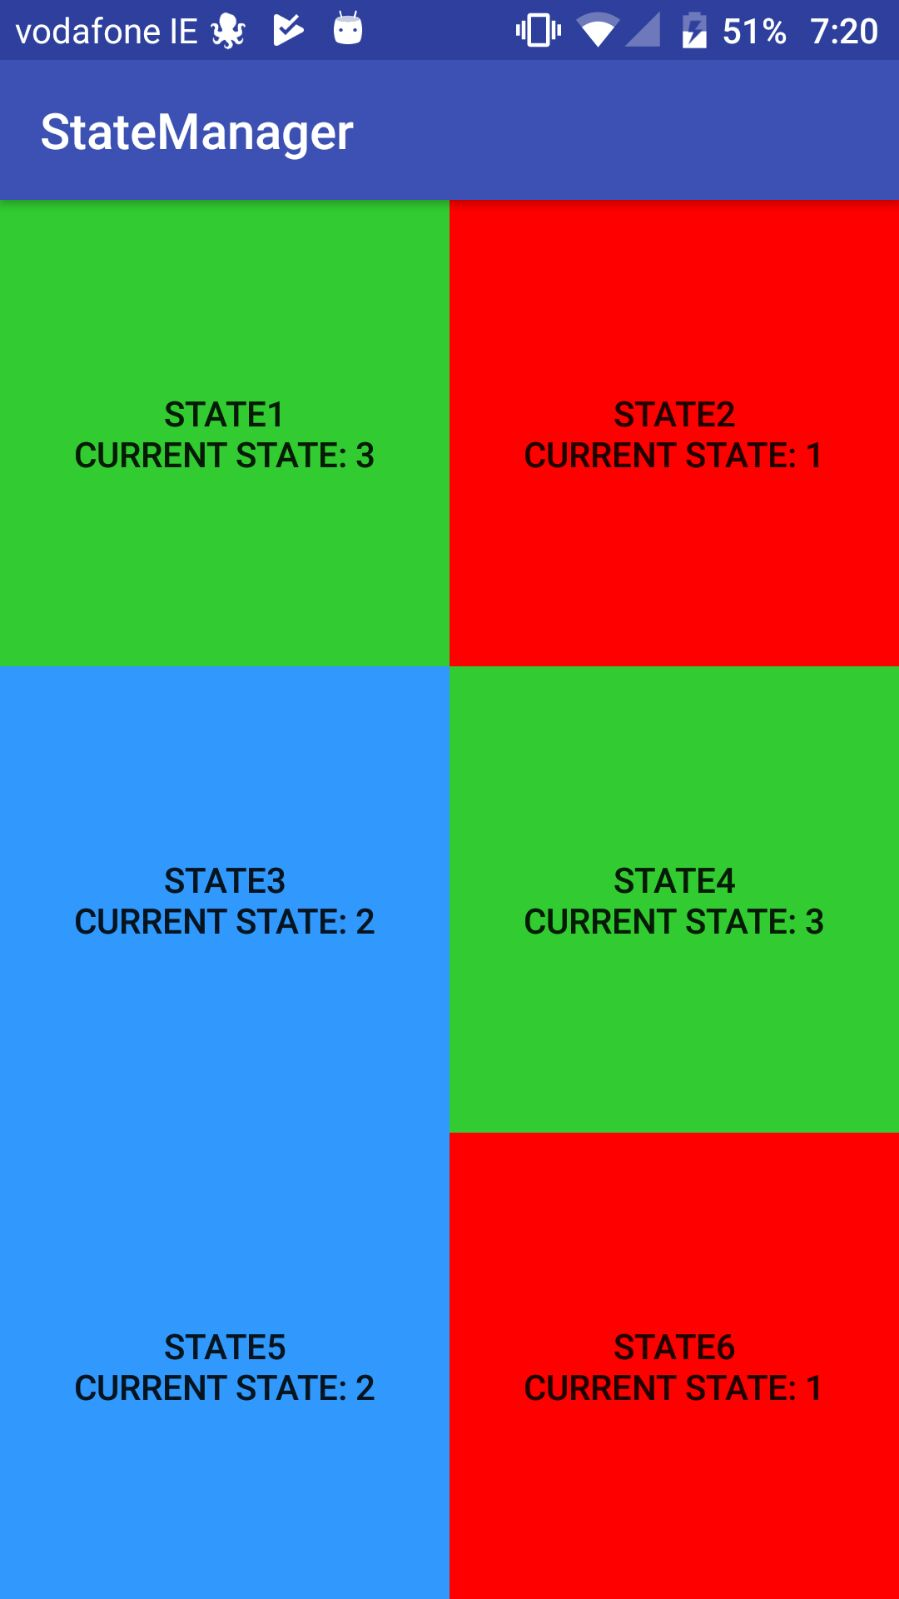
\includegraphics[width=0.7\textwidth,height=0.7\textheight]{android-agent}
\end{center}
A screenshot of the android agent and its state based tiles.
\end{tcolorbox}
\caption{Android agent for Iris}
\end{figure}

\subsubsection{Linkage with Iris}
The android application is linked to Iris through a unique REST endpoint specific to the android agent schema. All of the data being sent from the android application is sent to this endpoint. Once the data enters Iris, Iris will run through it's logic for checking for dashboards and charts associated with the schema and send the data through to the charts. 
%Add a ref to a section where you explain what iris does, so you dont have to keep repeating this for all agents
In this case the charts are state based and will update according to the state values that are given to them.

\begin{figure}[H]
\begin{tcolorbox}
\begin{center}
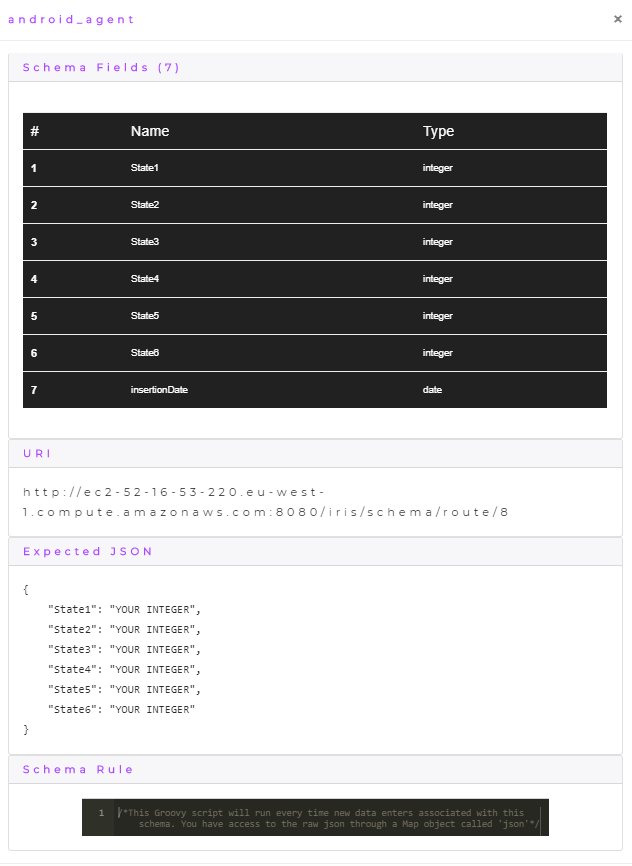
\includegraphics[width=\textwidth,height=\textheight,keepaspectratio]{iris-android-schema}
\end{center}
A screenshot of the Android agent schema in Iris
\end{tcolorbox}
\caption{Android agent schema in Iris}
\end{figure}

%Iris Android agent dashboard screenshot
\begin{figure}[H]
\begin{tcolorbox}
\begin{center}
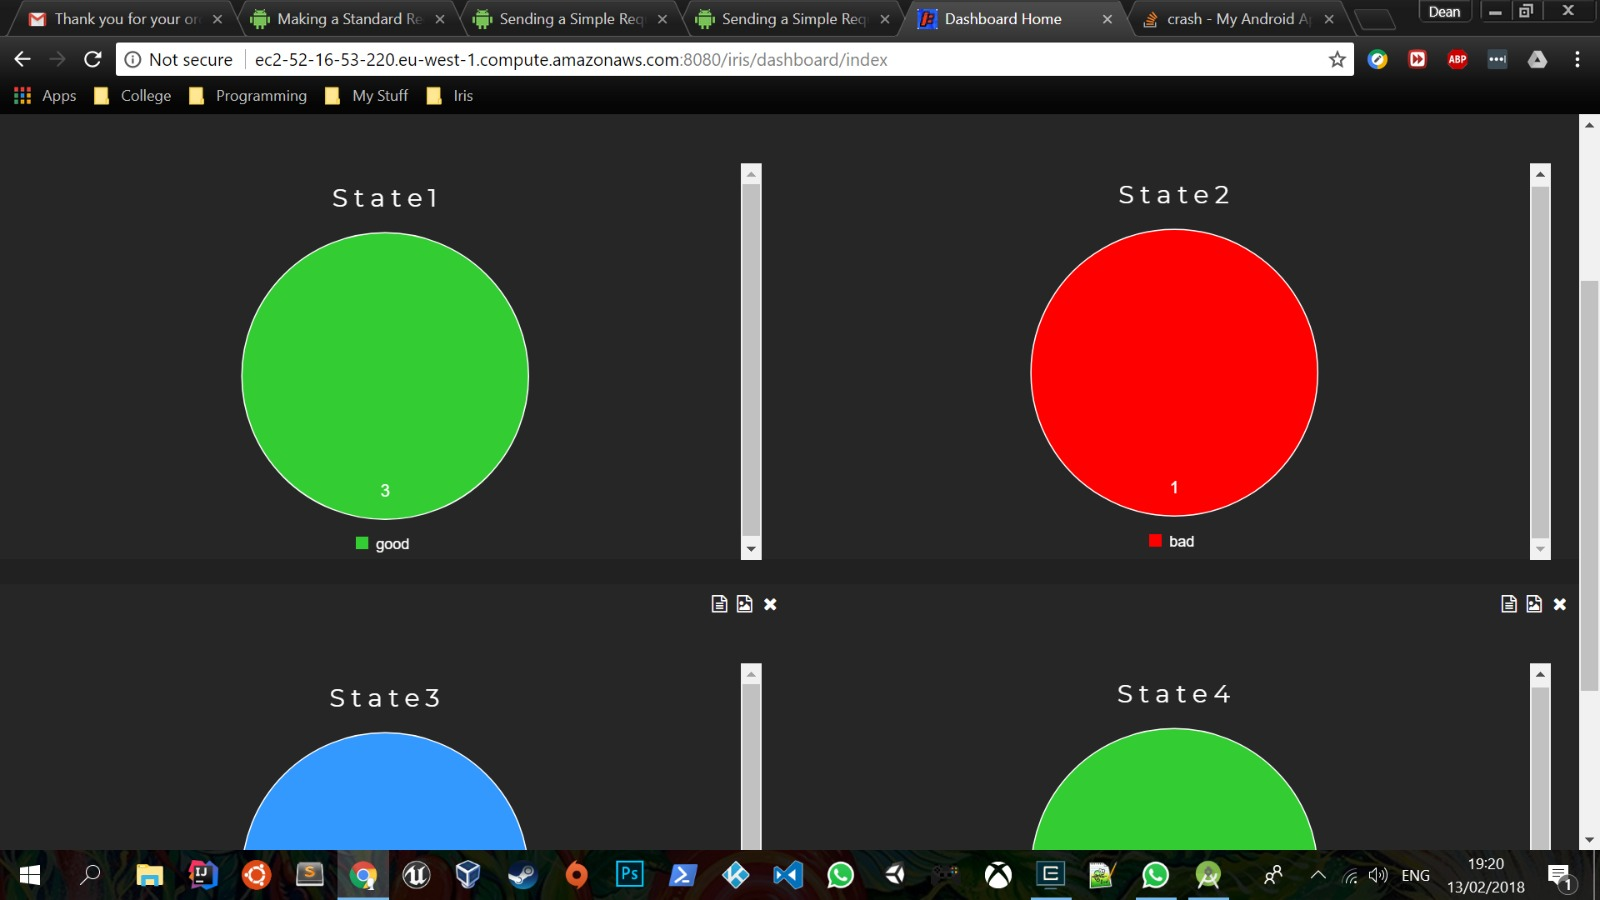
\includegraphics[width=\textwidth,height=\textheight,keepaspectratio]{iris-android-dashboard}
\end{center}
A screenshot of the android agent dashboard in Iris and its state based tiles.
\end{tcolorbox}
\caption{Android agent dashboard in Iris}
\end{figure}


\subsection{Raspberry Pi}
The Raspberry Pi agent is used to demonstrate the plug and play ability of a Raspberry Pi combined with the versatility of Iris.

\subsubsection{Description}
The Raspberry Pi agent demonstrates how a user can use a Raspberry Pi to run a script to continuously monitor an API. In the case the Raspberry Pi monitors crypto currency exchange rates using a python script through a library called `coinmarketcap'. The python script simply retrieves the latest crypto currency data through the `coinmarketcap' library and sends the data to the corresponding `crypto\_agent' endpoint in Iris. The Raspberry Pi agent is configured to run the script every minute with crontab and is also configured to automatically sign in to the terminal. This results in a plug and play agent wherever their is a network cable available.

%Crypto-currency script
\begin{figure}[H]
\begin{tcolorbox}
\begin{minted}{python}
#!/usr/bin/python

import requests, json
from coinmarketcap import Market

headers = {'Content-type': 'application/json', 'Accept': 'text/plain'}

agentData = {'name': 'crypto_agent'}

urlResp = requests.post('http://ec2-52-16-53-220.eu-west-1.compute.'+
'amazonaws.com:8080/iris/schema/getAgentUrl', 
data=json.dumps(agentData), headers=headers)

endpoint = urlResp.json()['url']

wanted_keys = ['price_usd', 'price_eur','name', 
               'percent_change_24h', 'rank']

def extract(data):
    return dict((k, data[k]) for k in wanted_keys if k in data)

coinmarketcap = Market()

crypto_currencies = coinmarketcap.ticker(limit=4, convert='EUR')

filterd_currencies = list(map(extract, crypto_currencies))

for currency in filterd_currencies:
    resp = requests.post(endpoint, 
                         data=json.dumps(currency), 
                         headers=headers)
    print resp.json()
\end{minted}
\end{tcolorbox}
\caption{Raspberry Pi Agent, iris-crypto-rates.py source code}
\end{figure}

For more information on coinmarketcap see their site here \url{https://coinmarketcap.com/}

\subsubsection{Linkage with Iris}
The Raspberry Pi agent is linked to Iris through a unique REST endpoint specific to the Raspberry Pi agent schema. All of the data being sent from the Raspberry Pi is sent to this endpoint. Once the data enters Iris, Iris will run through it's logic for checking for dashboards and charts associated with the schema and send the data through to the charts. 
%Add a ref to a section where you explain what iris does, so you dont have to keep repeating this for all agents
In this case Iris is monitoring raw data on two charts that are monitoring the current price in euro and usd. The other charts are using Elasticsearch aggregations to monitor the min and max prices reached for currencies in both euro and usd.

%Raspberry Pi agent schema screenshot in Iris
\begin{figure}[H]
\begin{tcolorbox}
\begin{center}
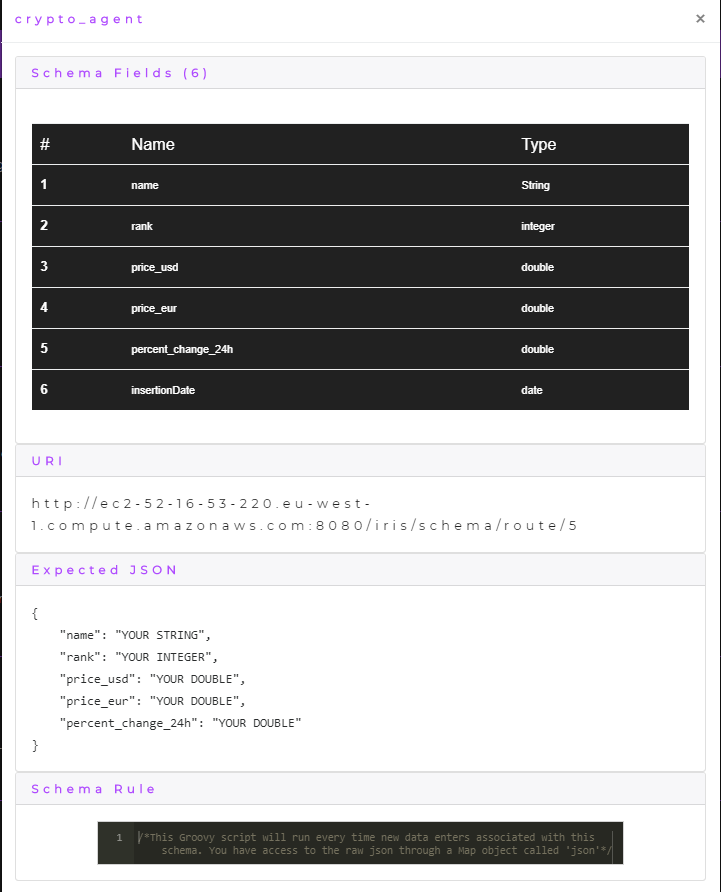
\includegraphics[width=\textwidth,height=\textheight,keepaspectratio]{iris-crypto-schema}
\end{center}
A screenshot of the Raspberry Pi agent schema in Iris
\end{tcolorbox}
\caption{Raspberry Pi agent schema in Iris}
\end{figure}

%Iris Raspberry Pi agent dashboard screenshot
\begin{figure}[H]
\begin{tcolorbox}
\begin{center}
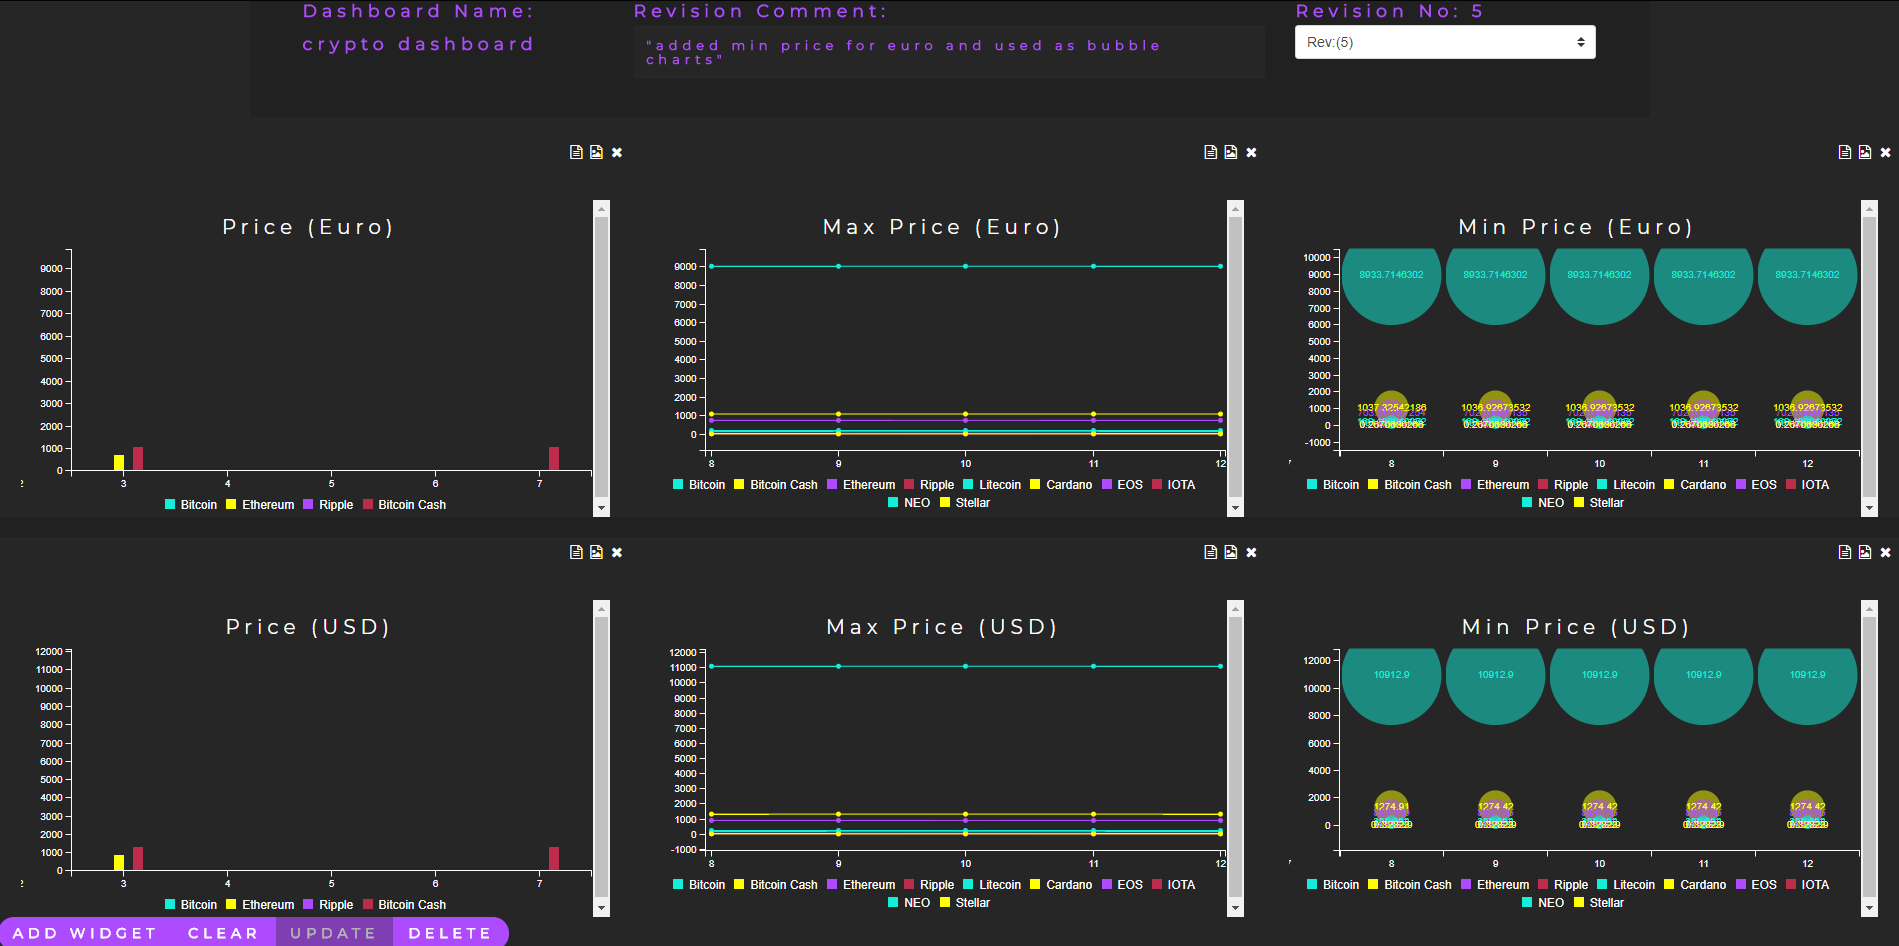
\includegraphics[width=\textwidth,height=\textheight,keepaspectratio]{iris-crypto-agent-dashboard}
\end{center}
A screenshot of the Raspberry Pi agent dashboard in Iris monitoring crypto currencies
\end{tcolorbox}
\caption{Raspberry Pi agent dashboard in Iris}
\end{figure}

\subsection{Node.js}
The Node.js agent shows how Iris can integrate with one of the most popular server-side frameworks and how it can monitor the status of the system running Node.js through the npm (node package manager) package `systeminformation'.

\subsubsection{Description}
Due to Node.js' rise in popularity in recent years this agent demonstrates how Iris can easily monitor a system using the `systeminformation' package from npm. The `systeminformation' package offers various levels of detail about the system running Node. Iris' schema for the Node.js agent measures the following attributes:
\begin{itemize}
    \item Operating System Name
    \item Current Uptime of the Operating System
    \item Current CPU Speed
    \item Total Memory Available
    \item Total Memory Free
    \item Total Memory Used
    \item Current CPU Load
\end{itemize}
A full list of all the obtainable attributes through `systeminformation' can be found here \url{https://github.com/sebhildebrandt/systeminformation}.

An important thing to note about this agent is that it takes use of Iris' ability to transform incoming data through scripting. Many of the memory attributes retrieved from `systeminformation' are represented in bytes, this agent uses Iris' centralised transformation abilities to transform the `memFree' attribute to be represented as gigabytes rather than bytes. This script also transforms all the `osName' attributes to be uppercase. Transforming these attributes in Iris through scripting removed the need for a redeployment of the Node.js application.

%Node.js agent transformation script
\begin{figure}[H]
\begin{tcolorbox}
\begin{center}
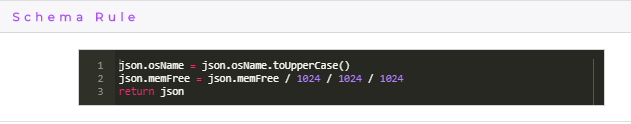
\includegraphics[width=\textwidth,height=\textheight,keepaspectratio]{node-transformation-script}
\end{center}
The transformation script for the Node.js agent which turns the `osName' attribute to uppercase and the `memFree' attribute to be gigabytes rather than bytes.
\end{tcolorbox}
\caption{Node.js agent transformation script}
\end{figure}

\subsubsection{Linkage with Iris}
The Node.js agent is linked to Iris through a unique REST endpoint specific to the Node.js agent schema. All of the data being sent from the Node.js agent is sent to this endpoint. Once the data enters Iris, Iris will run through it's logic for checking for dashboards and charts associated with the schema and send the data through to the charts. 
%Add a ref to a section where you explain what iris does, so you dont have to keep repeating this for all agents
In this case Iris is monitoring raw data on three charts that are monitoring the current memory free in gigabytes, the current memory used and the current uptime of the system. The other charts display the max memory used over all operating systems and the pie chart shows all the types of operating systems which have run the agent, both of these use Elasticsearch aggregations to calculate the data for the charts.

%Node.js agent schema screenshot in Iris
\begin{figure}[H]
\begin{tcolorbox}
\begin{center}
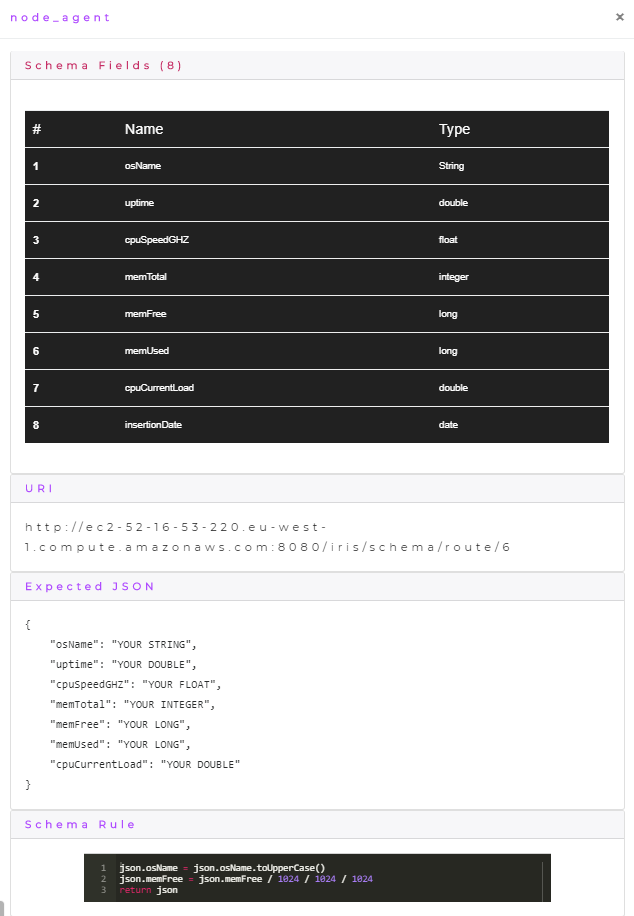
\includegraphics[width=\textwidth,height=\textheight,keepaspectratio]{iris-node-schema}
\end{center}
A screenshot of the Node.js agent schema in Iris
\end{tcolorbox}
\caption{Node.js agent schema in Iris}
\end{figure}

%Iris Node agent dashboard screenshot
\begin{figure}[H]
\begin{tcolorbox}
\begin{center}
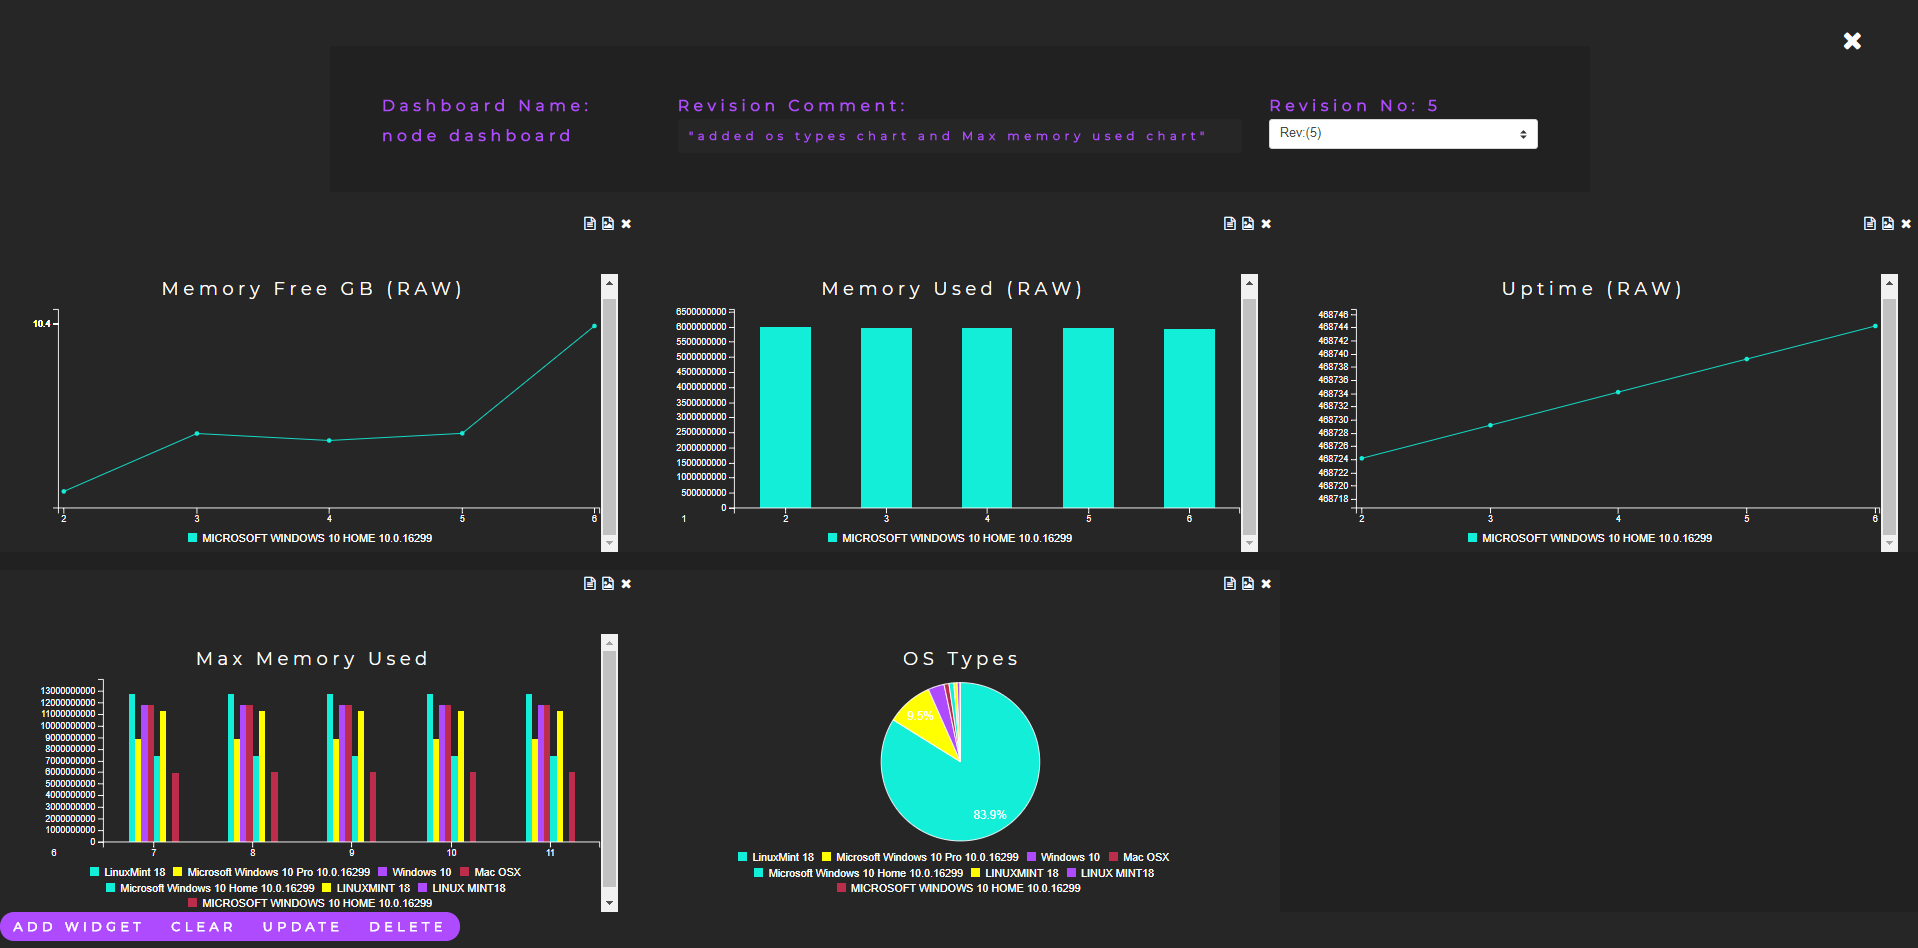
\includegraphics[width=\textwidth,height=\textheight,keepaspectratio]{iris-node-agent-dashboard}
\end{center}
A screenshot of the Node.js agent dashboard in Iris monitoring system information
\end{tcolorbox}
\caption{Node.js agent dashboard in Iris}
\end{figure}


\subsection{Selenium}
The Selenium agent demonstrates the versatility of Iris by monitoring the price of a guitar by scraping music store websites and monitoring the price of the guitar. This agent focuses on versatility over complexity.
\subsubsection{Description}
The Selenium agent demonstrates Iris' versatility through the Selenium web driver which is commonly used for web automation and functional testing. In this case Selenium is used in conjunction with a Selenium wrapper called `Selenide' to automate the scraping of music store websites for a specific guitar. On each site the guitar's price is taken from the webpage as well as the name of the music store, the price of the guitar and the name of the music store is then sent to Iris so that it may be monitored.

For more information on Selenide see their site here \url{http://selenide.org/}

\subsubsection{Linkage with Iris}
The Selenium agent is linked to Iris through a unique REST endpoint specific to the Selenium agent schema. All of the data being sent from the Selenium agent is sent to this endpoint. Once the data enters Iris, Iris will run through it's logic for checking for dashboards and charts associated with the schema and send the data through to the charts. 
%Add a ref to a section where you explain what iris does, so you dont have to keep repeating this for all agents
In this case Iris is monitoring raw data on a bar chart. The bar chart monitors the price of the guitar in euro and labels the chart based on the music store website that the price has been scraped from. In this case two sites have been scraped `Thomann' and `MusicStore.de', both sites are competitors and this reflects in the chart as both sites have matched the price of the guitar at the same price.

%Iris selenium agent schema screenshot
\begin{figure}[H]
\begin{tcolorbox}
\begin{center}
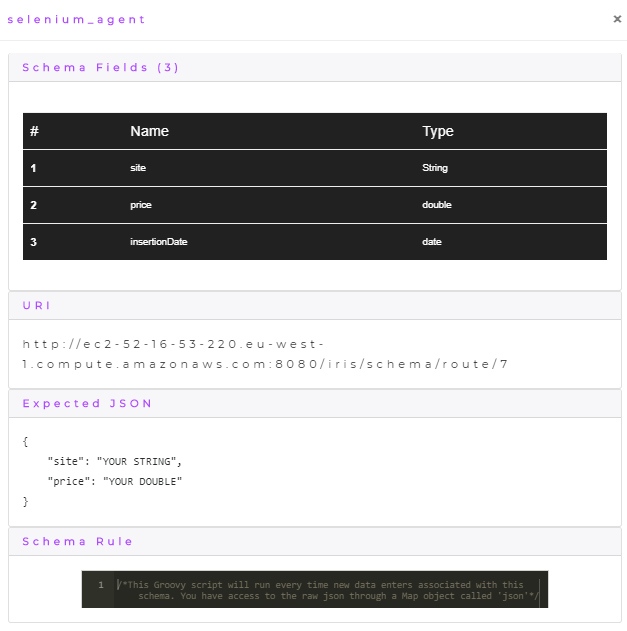
\includegraphics[width=\textwidth,height=\textheight,keepaspectratio]{iris-selenium-schema}
\end{center}
A screenshot of the Selenium agent schema in Iris
\end{tcolorbox}
\caption{Selenium agent schema in Iris}
\end{figure}

%Iris selenium agent dashboard screenshot
\begin{figure}[H]
\begin{tcolorbox}
\begin{center}
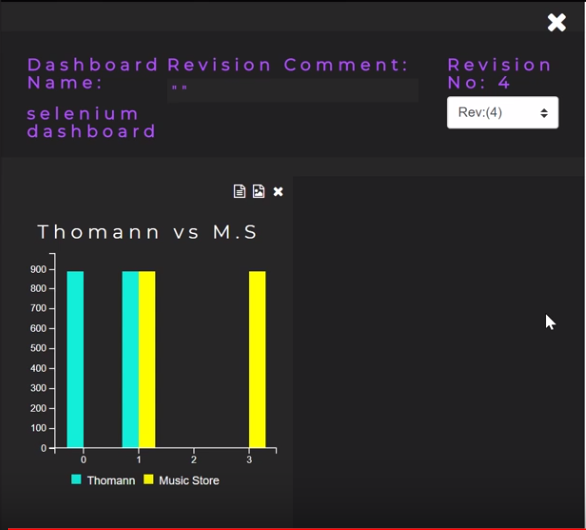
\includegraphics[width=\textwidth,height=\textheight,keepaspectratio]{iris-selenium-dashboard}
\end{center}
A screenshot of the Selenium agent dashboard in Iris
\end{tcolorbox}
\caption{Selenium agent dashboard in Iris}
\end{figure}

\subsection{MySQL}
The MySQL agent demonstrates how a user can monitor their database by converting the MySQL `information\_schema' results into JSON and sending them to Iris.
\subsubsection{Description}
The MySQL agent is significant for Iris as this agent was the inspiration for Iris in the beginning, as Onaware developers wanted a way to monitor a remote MySQL database with scripts and be able to monitor the database memory locally with a web application. The MySQL agent is a simple python script that connects to the MySQL instance and monitors all the databases as well as the amount of memory they use. The database name and the amount of memory it currently uses is then sent to Iris to be monitored. The python script is run every day at 8:00pm on the same AWS server that Iris is running on using a cron job.

%Crypto-currency script
\begin{figure}[H]
\begin{tcolorbox}
\begin{minted}{mysql}
SELECT table_schema AS "databaseName", 
ROUND(SUM(data_length + index_length) / 1024 /  1024, 2) as "memoryMB" 
FROM information_schema.TABLES 
GROUP BY table_schema;
\end{minted}
\end{tcolorbox}
\caption{MySQL Agent, MySQL `information\_schema' table query used in iris-mysql.py source code}
\end{figure}

More information on the MySQL `information\_schema' table can be found here \url{https://dev.mysql.com/doc/refman/5.7/en/information-schema.html}


\subsubsection{Linkage with Iris}
The MySQL agent is linked to Iris through a unique REST endpoint specific to the MySQL agent schema. All of the data being sent from the MySQL agent is sent to this endpoint. Once the data enters Iris, Iris will run through it's logic for checking for dashboards and charts associated with the schema and send the data through to the charts. 
%Add a ref to a section where you explain what iris does, so you dont have to keep repeating this for all agents
The MySQL agent dashboard monitors the average memory taken up by each database in the MySQL instance and displays the results as a line chart in Iris.
%Iris mysql schema screenshot
\begin{figure}[H]
\begin{tcolorbox}
\begin{center}
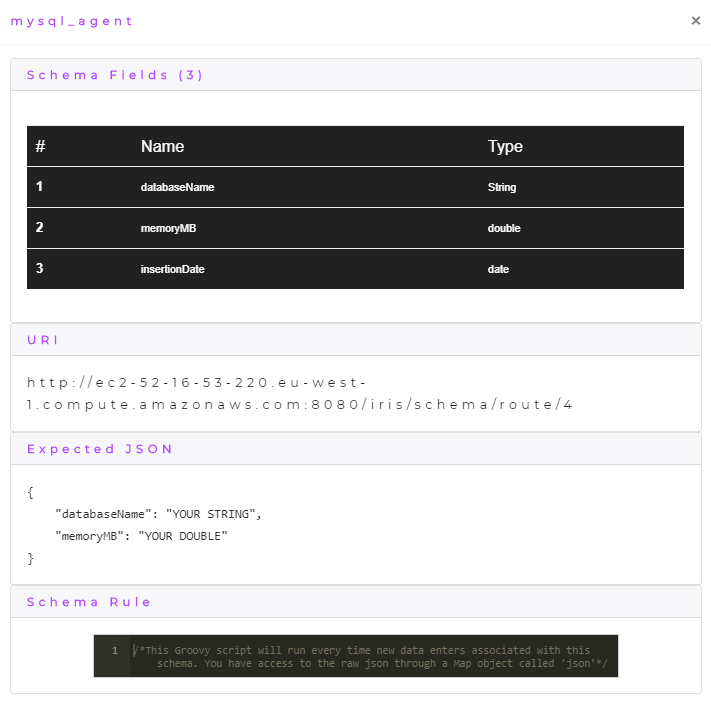
\includegraphics[width=\textwidth,height=\textheight,keepaspectratio]{iris-mysql-schema}
\end{center}
A screenshot of the MySQL agent schema in Iris
\end{tcolorbox}
\caption{MySQL agent schema in Iris}
\end{figure}

%Iris mysql dashboard screenshot
\begin{figure}[H]
\begin{tcolorbox}
\begin{center}
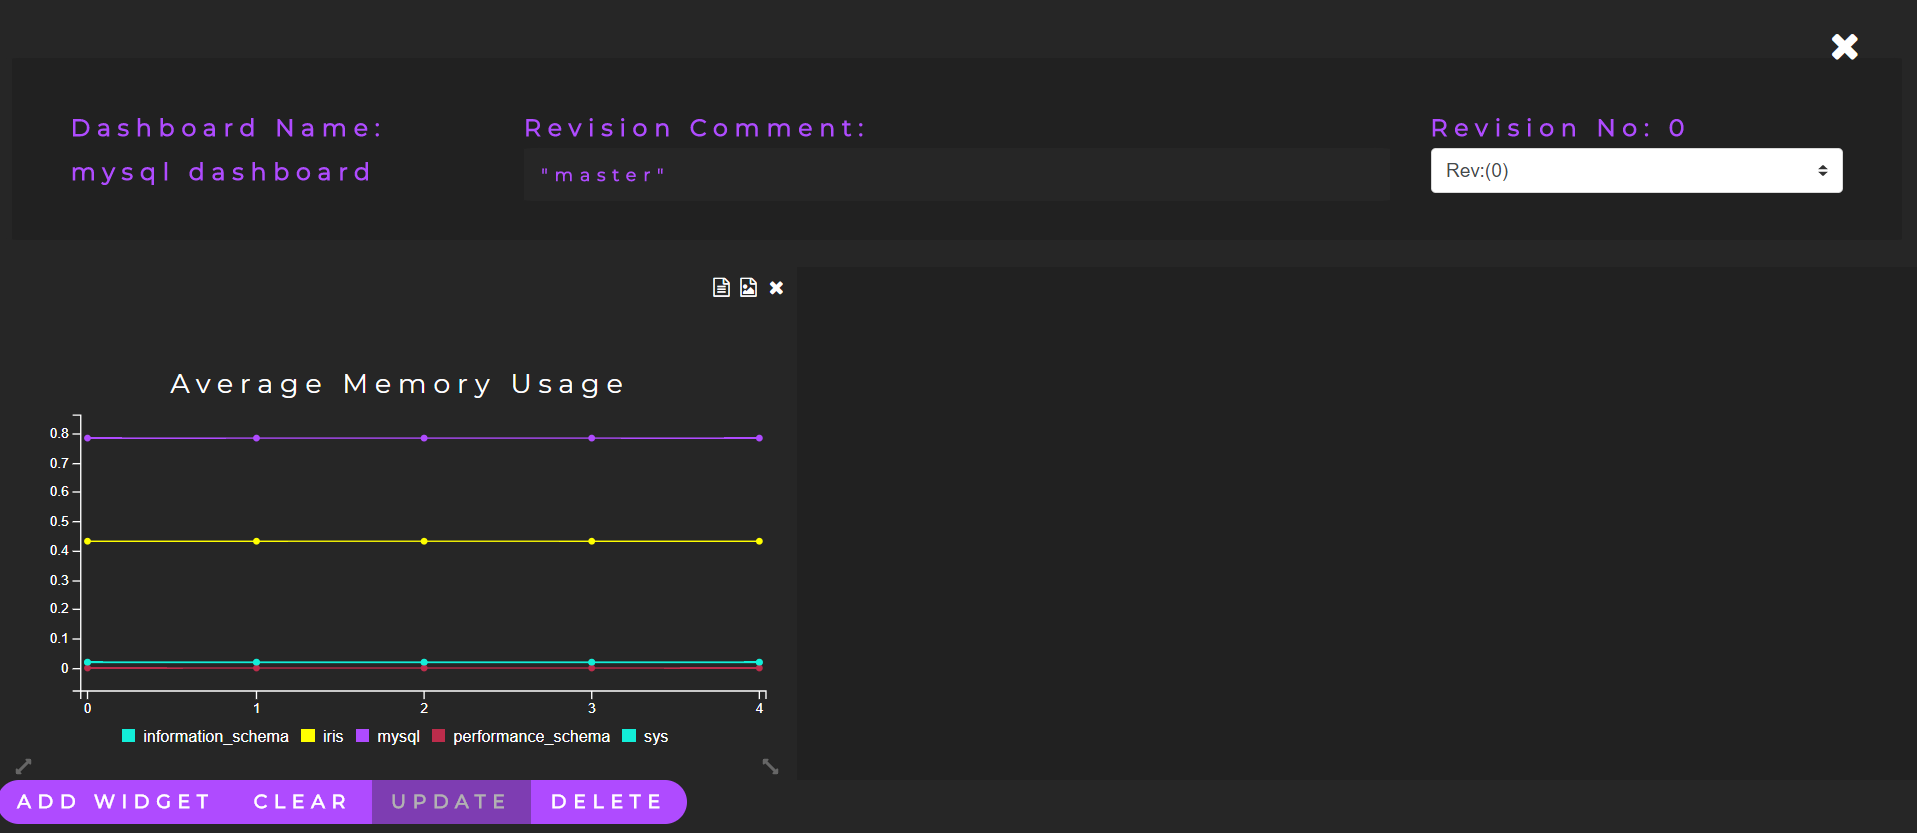
\includegraphics[width=\textwidth,height=\textheight,keepaspectratio]{iris-mysql-dashboard}
\end{center}
A screenshot of the MySQL agent dashboard in Iris
\end{tcolorbox}
\caption{MySQL agent dashboard in Iris}
\end{figure}

\chapter{Conclusions}


%No cite prints all references even if they are not in the document!!
\nocite{*}
\printbibliography

%%%%%%%%%%%%%%%%%%%%%%%%%%%%%%%%
\clearpage

\begin{appendices}

\end{appendices}
\end{document}
